\documentclass[12pt, a4paper, twoside]{article}

\usepackage[utf8]{inputenc}
\usepackage{amsmath}
\usepackage{amssymb}
\usepackage{physics}
\usepackage{pgfplots}
\usepackage{mathtools}

\title{Modelling the oscillation of walking humans}
\author{Martin Velikov}
\date{August 2022}

\begin{document}

% title & contents
\maketitle
\tableofcontents

% content
\section{Introduction}
\subsection{Aim}
The aim of this investigation is, using mathematical functions, to model the
vertical oscillation of the human body while walking.

\subsection{Applications}
There are numerous applications of modern technology where being able to model the
oscillation from walking is invaluable. For example, optical image stabilization
present in nearly all modern video cameras aims to minimize the 'screen shake' by
compensating with movement in the lens of the camera. A model of oscillation while
walking could aid this endeavor by allowing more predictable corrections to be made
by software.

\section{Least Squares Fitting}
\subsection{Theory}

Suppose that there is a polynomial $P$ of degree $k$ so that
\begin{align*}
    P(x)= a_0 + a_1 x + \cdots + a_{k-1} x^{k-1} + a_k x^k
\end{align*}

The coefficients $a_0$ through $a_k$ are the unknowns that must be solved for,
defining the shape of the polynomial. Assuming one wants to fit this polynomial
to a set of points, it would be useful to know how accurately a polynomial with
a guess of the coefficients $a_0 \cdots a_k$  can model the dataset. \\

\begin{figure}[!h]
    \centering
    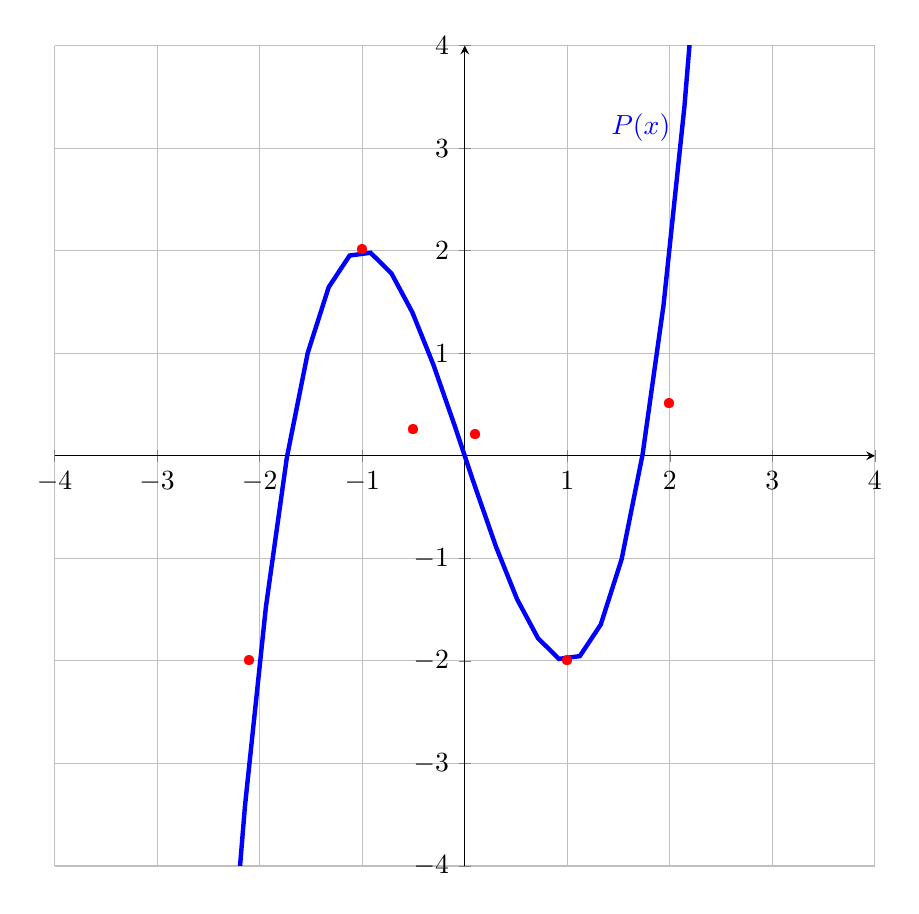
\begin{tikzpicture}
        \begin{axis}[
                axis y line=center,
                axis x line=middle,
                xmin=-4,
                xmax=4,
                ymin=-4,
                ymax=4,
                height=12.0cm,
                width=12.0cm,
                grid,
                xtick={-4,...,4},
                ytick={-4,...,4},
            ]
            \addplot [domain=-5:5, samples=50, mark=none, ultra thick, blue] {x^3-3*x};
            \node [left, blue] at (axis cs: 2.1, 3.2) {$P(x)$};
            \node [red] at (axis cs: 1, -2) {\textbullet};
            \node [red] at (axis cs: 2, 0.5) {\textbullet};
            \node [red] at (axis cs: -0.5, 0.25) {\textbullet};
            \node [red] at (axis cs: -2.1, -2) {\textbullet};
            \node [red] at (axis cs: 0.1, 0.2) {\textbullet};
            \node [red] at (axis cs: -1, 2) {\textbullet};
        \end{axis}
    \end{tikzpicture}
    \caption{
        Example cubic ($k=3$) $P(x)$ fitting 5 points.
    }
\end{figure}

Let one of these points be represented as $(x, y)$. The vertical difference $r$ between this point and
the graph of $P$ could be simply represented by

\begin{align*}
    r=|y-P(x)|
\end{align*}

The absolute value of the difference is used, as $r$ should be indicative of the
deviation from the graph, the direction of difference is irrelevant.
Additionally, instead  of taking its modulus, it can simply be squared in order
to accentuate the error more, and be more  wieldy in the next parts.  This leaves
the final equation

\begin{align*}
    r=(y-P(x))^2
\end{align*}

The total measure of deviation $R^2$ from the graph $P(x)$, called the "residual",
can be obtained by summing up the aforementioned vertical differences for $n$
points with coordinates $(x, y)$:

\begin{align*}
    R^2 & = \sum^n_{i=1}[y_i-P(x_i)]^2 \\
    % &= \sum^n_{i=1}[
    %     y_i - (a_0 + a_1 x_i + \cdots + a_{k-1} x_i^{k-1} + a_k x_i^k)]^2
\end{align*}

The partial derivative of the residual with respect to each coefficient
can be found, and set to zero in order to ensure that coefficient contributes
a minimum of the error in terms of the entire equation. This results in the
following system of equations:

\begin{align*}
    \frac{\partial (R^2)}{\partial a_0}     & = -2 \sum^n_{i=1}[y_i-P(x_i)] x^0     & = 0 \\
    \frac{\partial (R^2)}{\partial a_1}     & = -2 \sum^n_{i=1}[y_i-P(x_i)] x^1     & = 0 \\
                                            & \vdotswithin{=}                             \\
    \frac{\partial (R^2)}{\partial a_{k-1}} & = -2 \sum^n_{i=1}[y_i-P(x_i)] x^{k-1} & = 0 \\
    \frac{\partial (R^2)}{\partial a_k}     & = -2 \sum^n_{i=1}[y_i-P(x_i)] x^k     & = 0
\end{align*}

These can be expanded, and made into a system of equations, then represented as
matrices for a solution. The proof of this, however, is beyond the scope of this
investigation. After simplification, the matrix system can be represented as

\begin{align*}
    \begin{bmatrix}
        1      & x_1     & x_1^2     & \cdots & x_1^{k-1}     & x_1^k     \\
        1      & x_2     & x_2^2     & \cdots & x_2^{k-1}     & x_2^k     \\
        \vdots & \vdots  & \vdots    & \ddots & \vdots        & \vdots    \\
        1      & x_{n-1} & x_{n-1}^2 & \cdots & x_{n-1}^{k-1} & x_{n-1}^k \\
        1      & x_n     & x_n^2     & \cdots & x_n^{k-1}     & x_n^k
    \end{bmatrix}
    \begin{bmatrix}
        a_1 \\ a_2 \\ \vdots \\ a_{k-1} \\ a_k
    \end{bmatrix}
    =
    \begin{bmatrix}
        y_1 \\ y_2 \\ \vdots \\ y_{n-1} \\ y_n
    \end{bmatrix}
\end{align*}

An interesting point about this method is that if the number of points $n$ that
the polynomial must be fit to exceeds the degree $k$, the polynomial can never pass
through all of them exactly. This means that the above system of patrices is
"over-determined", that is, it can never give a perfect solution, only the
closest approximation. \\

Multiplying by the transpose $X^T$ of the matrix with x-terms $X$ would yield
a square linear system which can then be solved numerically for the coefficients in the
vector $\vec{a}$.

\begin{align*}
    X^TX\vec{a}=X^T\vec{y}
\end{align*}

As mentioned above, and in the case that applies to solving this problem, a well-formed
solution to this system does not exist most of the time. However, if the degree $k$
is greater than $n$, the system can be solved for a
single vector of solutions.

\begin{align*}
    \vec{a}=(X^TX)^{-1}X^T\vec{y}
\end{align*}

\end{document}